\documentclass{article} % For LaTeX2e
\usepackage{nips15submit_e,times}
\usepackage{hyperref}
\usepackage{graphicx}
\usepackage{hyperref}
\usepackage{url}
\usepackage{times}
\usepackage{epsfig}
\usepackage{graphicx}
\usepackage{amsmath}
\usepackage{amssymb}
\usepackage{multirow}
\usepackage{caption} 
\usepackage{url}
%\documentstyle[nips14submit_09,times,art10]{article} % For LaTeX 2.09

\title{Normalisation aux batches des resaux neurales recurrents}

\author{
Me \\
\And
Nicolas \\
\And
C\'esar \\
\And
Aaron
\texttt{email} \\
}

\newcommand{\fix}{\marginpar{FIX}}
\newcommand{\new}{\marginpar{NEW}}

%\nipsfinalcopy % Uncomment for camera-ready version

\usepackage{amsfonts}
\usepackage{amsmath}

\newcommand{\vect}[1]{\mathbf{#1}}
\newcommand{\mat}[1]{\mathbf{#1}}
\newcommand{\act}{f}
\newcommand{\ewprod}{\odot}
\newcommand{\reals}{\mathbb{R}}
\newcommand{\given}{\vert}

\begin{document}

\maketitle

\begin{abstract}
\,Ca marche!
\end{abstract}

\section{Introduction}

[Given ill-conditioning, acceptable optimization can still be obtained by better optimization algorithms, such as
Hessian-Free~\cite{hessianfree} or the various approximations to natural gradient proposed in~\cite{ollivier} and~\cite{KFAC}.

Alternatively, the conditioning problem can also be addressed through model reparameterizations.
\cite{lecun}, \cite{raiko}, \cite{pascanu}, \cite{desjardins}.
batch normalization is one of these.]

Batch normalization~\cite{ioffe2015batch} greatly improves the training dynamics of deep feedforward neural networks, leading to faster convergence and better generalization.

However, applying batch normalization in recurrent neural networks has proven to be challenging.
In \cite{Baidu} batch normalization is applied in a stack of recurrent neural networks, but only to the input terms and not to the recurrent terms.
\cite{Cesar} 
Recently, a related technique called weight normalization~\cite{salimans2016weight} was introduced, which has a similar effect to batch normalization yet might be easier to carry over to the recurrent setting.

\section{Prerequisites}
\subsection{Recurrent neural networks}

Given an input sequence $\mat{X} = ( \vect{x}_1, \vect{x}_2, ... \vect{x}_T )$,

\begin{align}
\vect{h}_t = \mathrm{tanh}(
  \mat{W}_h \vect{h}_{t-1} +
  \mat{W}_x \vect{x}_t +
  \vect{b})
\end{align}

where $\mat{W}_h \in \reals^{d_h \times d_h},
       \mat{W}_x \in \reals^{d_x \times d_h},
       \vect{b} \in \reals^{d_h}$
  and the initial state $\vect{h}_0 \in \reals^{d_h}$
  are model parameters.

Recurrent neural networks are popular in sequence modeling tasks, as they naturally apply to variable-length sequences.

[optimization problems]
 the notorious training issues associated with recurrent neural networks, namely vanishing/exploding gradients~\cite{somebody} and the difficulty of learning long-term dependencies~\cite{somebody else}.

There exist a number of variants of the basic recurrent neural network given above, some specifically designed to address the problem of vanishing/exploding gradients, such as the Long Short-Term Memory (LSTM) unit~\cite{lstm} and Unitary RNNs~\cite{urnn}.

We will focus on LSTM, with recurrent transition given by

\begin{align}
\left(\begin{array}{ccc}
\vect{f}_t \\
\vect{i}_t \\
\vect{o}_t \\
\vect{g}_t
\end{array}\right)
 &=
\left(\begin{array}{ccc}
\sigma \\
\sigma \\
\sigma \\
\tanh
\end{array}\right)
\left(
 \mat{W}_h \vect{h}_{t-1} +
 \mat{W}_x \vect{x}_t +
 \vect{b}
\right) \\
\vect{c}_t &= \vect{f}_t \ewprod \vect{c}_{t-1} +
              \vect{i}_t \ewprod \vect{g}_t \\
\vect{h}_t &= \vect{o}_t \ewprod \tanh(\vect{c}_t)
\end{align}

where $\vect{W}_h \in \reals^{d_h \times 4 d_h}, \vect{W}_x \reals^{d_x \times 4 d_h}, \vect{b} \in \reals^{4 d_h}$ and the initial states $\vect{c}_0, \vect{h}_0 \in \reals^{d_h}$ are model parameters.
The $\ewprod$ operator denotes the elementwise product.

Intuitively, LSTM improves on the basic RNN in two ways.
First, it has an additional recurrent \emph{cell} state $\vect{c}_t$ whose recurrence is nearly linear, which allows gradient to flow backwards more easily.
Second, communication between this state and $\vect{h}_t$ and $\vect{x}_t$ is controlled by the gates $\vect{f}_t$, $\vect{i}_t$ and $\vect{o}_t$.

\subsection{Batch normalization}

Batch normalization is a simple reparameterization applied to neural network preactivations in order to make their distributions easier to control.
The batch normalizing transform is as follows:

\begin{align}
\mathrm{BN}(h; \gamma, \beta) =
  \beta + \gamma
  \frac{h -   \widehat{\mathrm{Mean}}(\mathcal{H})}
       {\sqrt{\widehat{\mathrm{Var }}(\mathcal{H}) + \epsilon}}
\end{align}

where $h \in \reals$ is the (pre)activation to be normalized, $\gamma \in \reals, \beta \in \reals$ are model parameters that determine the mean and standard deviation of the normalized activation, and $\epsilon \in \reals$ is a regularization hyperparameter.

$\mathcal{H}$ is distributed according to $p(\mathcal{H}|\mathcal{X}) p(\mathcal{X})$ with $p(\mathcal{X})$ being the data distribution.
At training time, the statistics $\mathrm{Mean}(\mathcal{H})$ and $\mathrm{Var}(\mathcal{H})$ are estimated by the sample mean and sample variance of the current minibatch.
This allows for backpropagation through the statistics, preserving the convergence properties of stochastic gradient descent.
During inference, the statistics are typically estimated based on the entire training set, to produce a deterministic prediction.

For notational convenience, we will denote by $\mathrm{BN}(\vect{x}; \vect{gamma}, \vect{beta})$ the elementwise normalization of activation vector $\vect{x}$.

Batch normalizing some hidden layer's activation ensures that its mean and variance are determined only by the $\beta$ and $\gamma$ parameters, and not by the parameters of any layer below it.
Applying this on every layer effectively decouples each layer's parameters from those of other layers, leading to a block-diagonal Fischer information matrix, and a better-conditioned optimization problem.
Deep neural networks trained with batch normalization converge significantly faster and generalize better.

\section{Recurrent batch normalization}

A recurrent neural network can be ``unrolled'' and viewed as a feedforward neural network.
This view suggests that the success of batch normalization in feedforward networks should carry over to the recurrent setting.
However, unrolled recurrent networks differ from true feedforward networks in several important respects that complicate the application of batch normalization.

\begin{itemize}
\item
The parameters in an unrolled recurrent network are shared across layers.
This suggests that the statistics used for normalization should be shared as well.
However, we have found that estimating the statistics independently at each timestep works best.
With batch normalization, the activations rapidly converge to a stationary distribution (cf. a figure), so independent estimation does not hurt performance.
Indeed, we find that sharing statistics does hurt performance, as the distribution of activations during the first few timesteps is very different from the stationary distribution.
\\ \item
The depth depends on the length of the input sequence $\mat{X} = (\vect{x}_t)$, which is typically not constant.
This poses a problem if we want to estimate the population statistics for different timesteps independently.
However, thanks to the stationarity of the activation distribution (cf. that figure) we can use the estimates of earlier timesteps for later timesteps.
For our experiments we estimate the population statistics separately for each timestep $1, \ldots, T_{max}$ where $T_{max}$ is the length of the longest training sequence.
When at test time we need to generalize beyond $T_{max}$, we use the population statistic of time $T_{max}$ for all time steps following it.

[there is an annoying little detail here: there may be only a single example with length T, and so the population statistic is highly unreliable. in this case i would take an earlier population statistic instead, the exact choice determined by validation. how do we explain this concisely?]
\\ \item
There is three-way interaction; each layer receives as input not just the activations of the layer below it but also the next element of the input sequence.
We find that we need to normalize these terms separately before adding them up.
This gives the model better control over the relative contribution of the terms.
\\ \item
The initial states $\vect{h}_0$ are independent of the input and thus have zero variance.
This problem is exacerbated in unnatural data such as MNIST and various pathological tasks, where some features are constant across the data.
In the sequential MNIST task in particular, the variance is typically exactly zero for the first hundred or so time steps, as the upper pixels are almost always black.
Normalizing these zero-variance activations involves division by a very small number at many timesteps, which causes the gradient to explode.
We work around this by injecting noise into the initial hidden states.
Although the normalization amplifies the noise to signal level, we find that it does not hurt performance compared to data-dependent ways of initializing the hidden states.
[but is that an artifact of classification at the end?]
\\ \item
Unrolled recurrent networks are typically much deeper than feedforward networks.
Rather than normalizing activations to have standard deviation 1, we normalize to standard deviation 0.1.
This avoids saturating the nonlinearities and enables better flow of gradients.
Indeed, we found that normalizing to unit variance caused the gradient to vanish rapidly.
[yet explode in LSTM...]
\end{itemize}

\subsection{Batch-normalized LSTM}

We introduce the batch normalizing transform $\mathrm{BN}(\cdot; \gamma, \beta)$ into the LSTM transition as follows:

\begin{align}
\left(\begin{array}{ccc}
\vect{f}_t \\
\vect{i}_t \\
\vect{o}_t \\
\vect{g}_t
\end{array}\right)
 &=
\left(\begin{array}{ccc}
\sigma \\
\sigma \\
\sigma \\
\tanh
\end{array}\right)
\left(
 \mathrm{BN} (\mat{W}_h \vect{h}_{t-1}; \vect{\gamma}_h, \vect{\beta}_h) +
 \mathrm{BN} (\mat{W}_x \vect{x}_t    ; \vect{\gamma}_x, \vect{\beta}_x) +
 \vect{b}
\right) \\
\vect{c}_t &= \vect{f}_t \ewprod \vect{c}_{t-1} +
              \vect{i}_t \ewprod \vect{g}_t \\
\vect{h}_t &= \vect{o}_t \ewprod \tanh(
 \mathrm{BN} (\vect{c}_t; \vect{\gamma}_c, \vect{\beta}_c)
)
\end{align}

Note how we normalize the recurrent term $\mat{W}_h \vect{h}_{t-1}$ and the input term $\mat{W}_x \vect{x}_t$ separately.
This allows the model to control the contribution of the two independently using $\vect{\gamma}_h$ and $\vect{\gamma}_x$.
To avoid unnecessary redundancy we set $\vect{\beta}_h = \vect{\beta}_x = \vect{0}$, instead relying on a single parameter vector $\vect{b}$ to account for both biases.

In order to leave the LSTM dynamics intact, we do not introduce batch normalization into the recurrence of the cell states.

During training we estimate the statistics needed for batch normalization across the minibatch, and independently for each timestep.
During inference we use estimates obtained by averaging the minibatch estimates both across the training set and across time.

\section{Experiments}

\subsection{Sequential MNIST}

\begin{figure}
\center
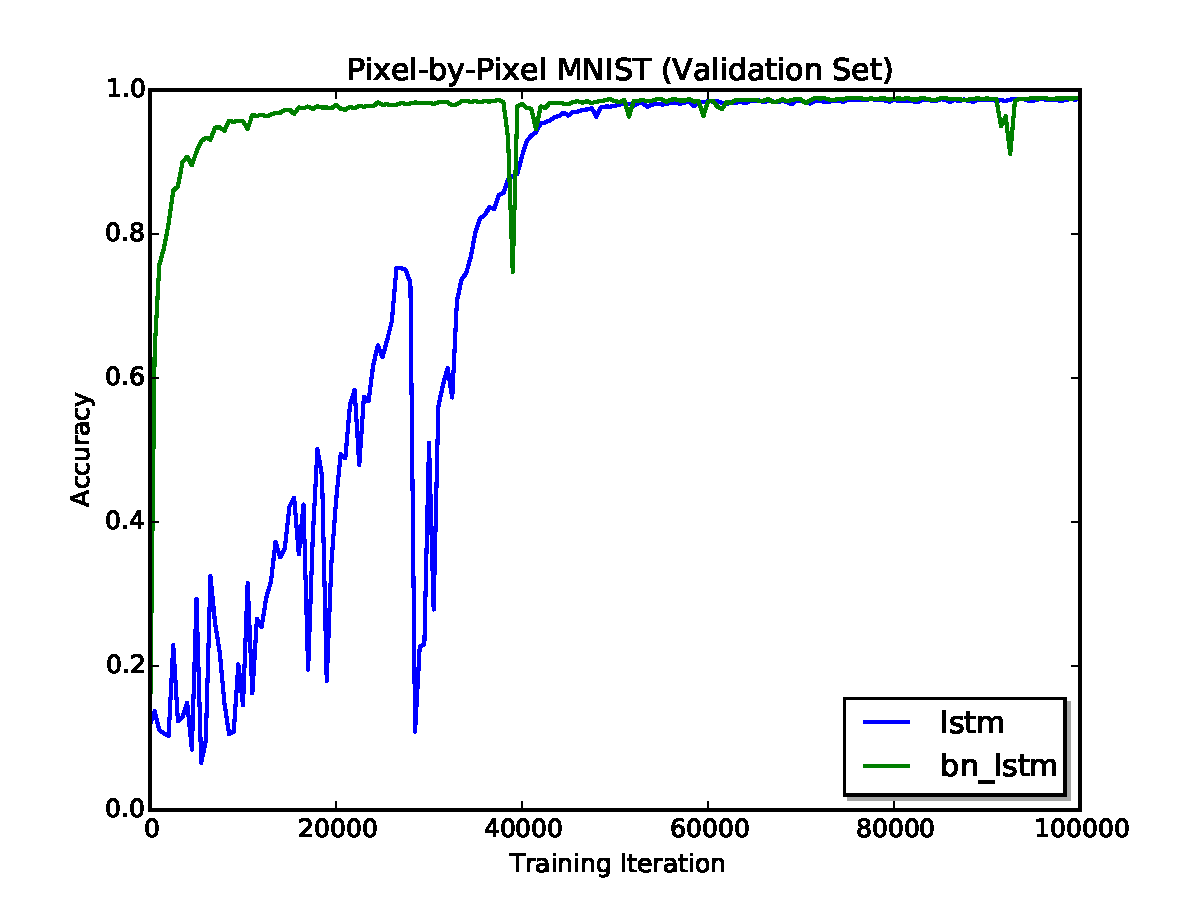
\includegraphics[width=7cm]{figures/unpermuted_valid.pdf}
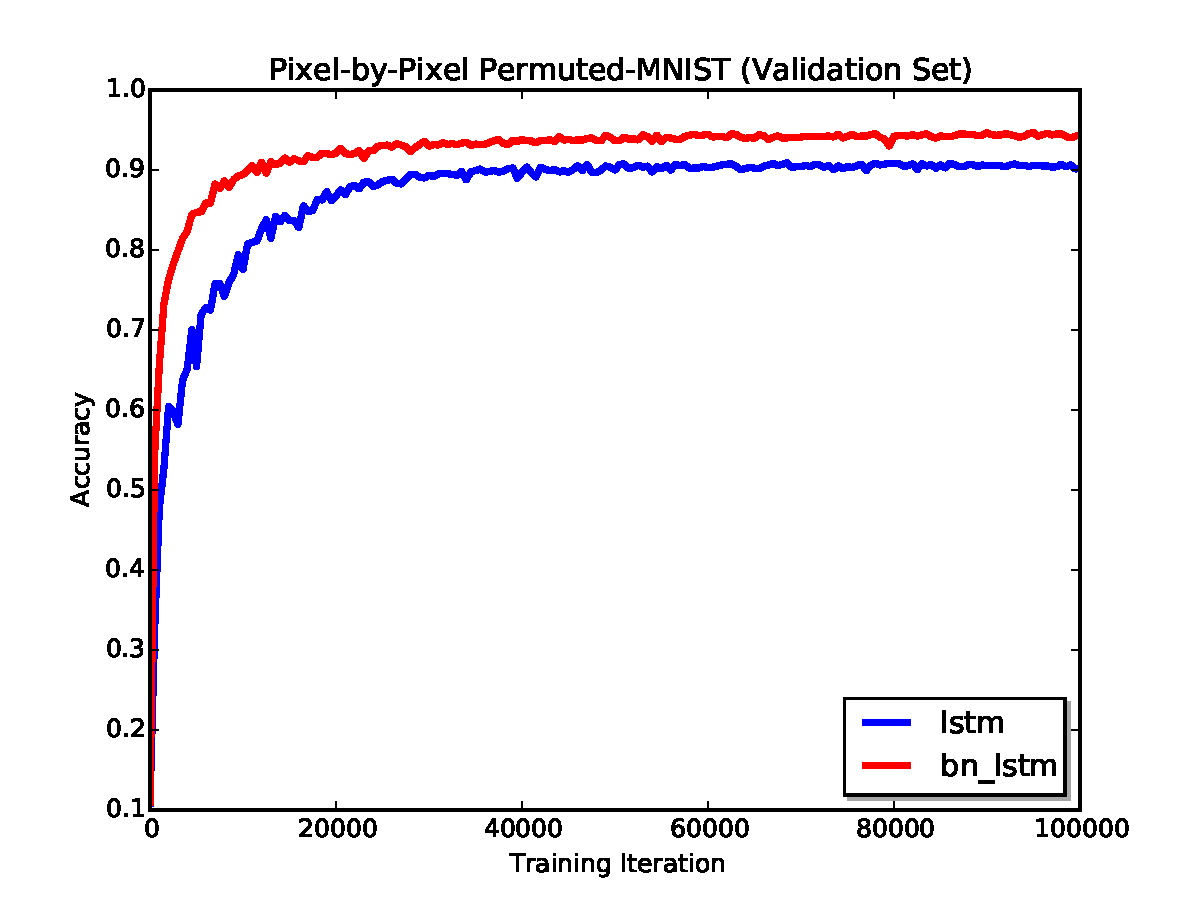
\includegraphics[width=7cm]{figures/permuted_valid.pdf}
\caption{Accuracy on the validation set for the pixel by pixel MNIST classification tasks. The batch-normalized LSTM is able to converge faster relatively to a baseline LSTM.
  Batch-normalized  LSTM also shows some improve generalization on the permuted sequential MNIST that require to preserve long-term memory information.}
\label{fig:seqmnist_valid}
\end{figure}


\begin{table}

\begin{tabular}{c|c|c}
   & UnPermuted & Permuted\\
  \hline
  LSTM & 98.8 & 90.1\\
  BN-LSTM & 99.0 & 95.1\\
\end{tabular}
\caption{Accuracy obtained on the test set for the pixel by pixel MNIST classification tasks}
\label{tab:seqmnist_test}

\end{table}

\subsection{Character-level Penn Treebank}

\subsection{TIMIT}

\subsection{Memory Networks}

\section{Conclusion}

\end{document}
